% Fig 3.19 Moessbauer effect: decay scheme 57Co -> 57Fe (I=5/2, 136 keV)
% -> I=3/2 (14.4 keV, 0.14 us) -> I=1/2 with branch ratios 9%/91%, resonant
% absorption in the absorber; below: source on a moving carriage with velocity v,
% gamma ray through the sample to the detector.
\documentclass[tikz,border=5pt]{standalone}
\usetikzlibrary{arrows.meta,decorations.pathmorphing}
\usepackage{amsmath}
\usepackage{bm}
\usepackage{fontspec}
\setmainfont{Times New Roman}
\begin{document}
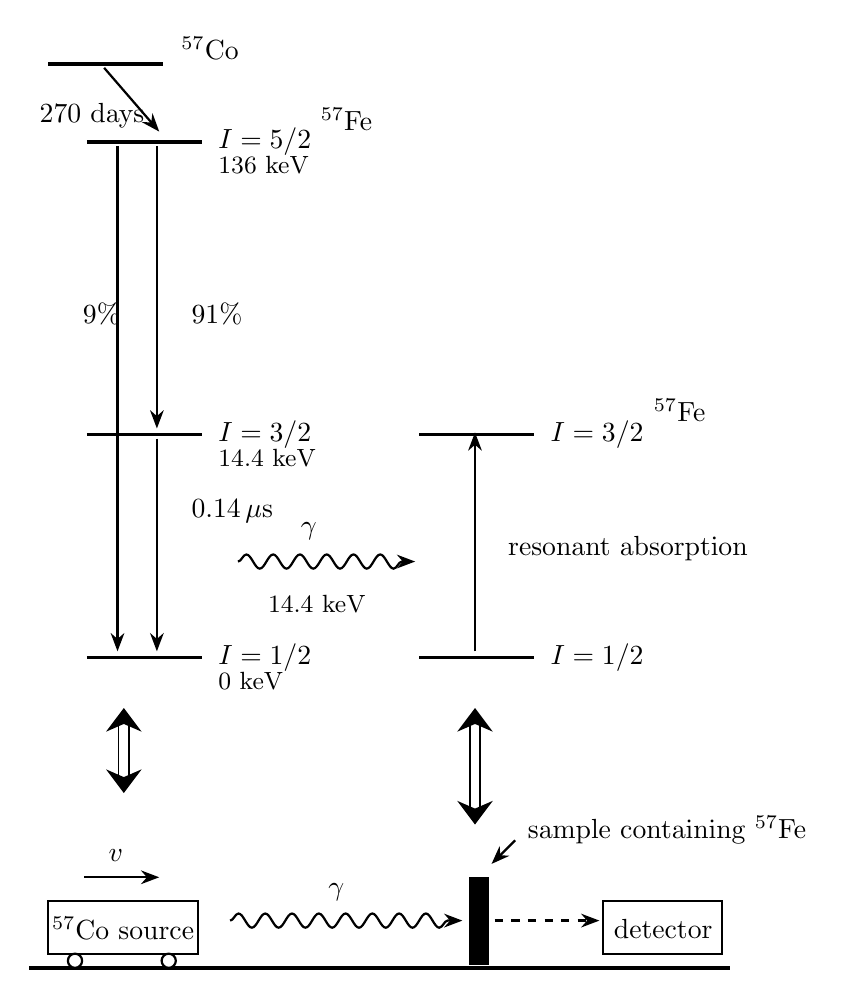
\begin{tikzpicture}[line width=0.8pt,>=Stealth,
  wv/.style={decorate,decoration={snake,amplitude=0.9mm,segment length=3.4mm,post length=1.6mm}}]
% ================= decay scheme =================
\draw[very thick] (0.29,11.58) -- (1.75,11.58);
\node[anchor=west] at (1.85,11.78) {$^{57}$Co};
\draw[->] (1.00,11.53) -- (1.70,10.72);
\node[anchor=west] at (0.05,10.92) {270 days};
% 57Fe I=5/2, 136 keV
\draw[very thick] (0.78,10.59) -- (2.24,10.59);
\node[anchor=west] at (2.32,10.59) {$I=5/2$};
\node[anchor=west] at (3.62,10.88) {$^{57}$Fe};
\node[anchor=west] at (2.32,10.30) {\small 136 keV};
% branches
\draw[->] (1.17,10.54) -- (1.17,4.12);
\node[anchor=west] at (0.60,8.40) {9\%};
\draw[->] (1.67,10.54) -- (1.67,6.95);
\node[anchor=west] at (1.98,8.40) {91\%};
% 57Fe I=3/2, 14.4 keV
\draw[very thick] (0.78,6.87) -- (2.24,6.87);
\node[anchor=west] at (2.32,6.87) {$I=3/2$};
\node[anchor=west] at (2.32,6.58) {\small 14.4 keV};
\draw[->] (1.67,6.82) -- (1.67,4.12);
\node[anchor=west] at (1.98,5.90) {0.14\,$\mu$s};
% 57Fe I=1/2, 0 keV
\draw[very thick] (0.78,4.04) -- (2.24,4.04);
\node[anchor=west] at (2.32,4.04) {$I=1/2$};
\node[anchor=west] at (2.32,3.75) {\small 0 keV};
% gamma photon and absorber levels
\draw[wv,->] (2.70,5.26) -- (4.95,5.26);
\node at (3.60,5.65) {$\gamma$};
\node at (3.70,4.72) {\small 14.4 keV};
\draw[very thick] (5.00,6.87) -- (6.46,6.87);
\node[anchor=west] at (6.54,6.87) {$I=3/2$};
\node[anchor=west] at (7.85,7.18) {$^{57}$Fe};
\draw[very thick] (5.00,4.04) -- (6.46,4.04);
\node[anchor=west] at (6.54,4.04) {$I=1/2$};
\draw[->] (5.71,4.12) -- (5.71,6.90);
\node[anchor=west] at (6.00,5.42) {resonant absorption};
% ================= transition to experiment =================
\draw[{Stealth[length=3mm,width=4.5mm]}-{Stealth[length=3mm,width=4.5mm]},
      double distance=3.2pt,line width=0.5pt] (1.25,3.40) -- (1.25,2.32);
\draw[{Stealth[length=3mm,width=4.5mm]}-{Stealth[length=3mm,width=4.5mm]},
      double distance=3.2pt,line width=0.5pt] (5.71,3.40) -- (5.71,1.92);
% ================= experiment =================
\draw[very thick] (0.05,0.10) -- (8.95,0.10);
% source box on wheels
\draw (0.29,0.28) rectangle (2.19,0.95);
\node at (1.24,0.60) {$^{57}$Co source};
\draw[fill=white] (0.63,0.19) circle (0.09);
\draw[fill=white] (1.82,0.19) circle (0.09);
\draw[->] (0.75,1.25) -- (1.70,1.25);
\node at (1.15,1.52) {$v$};
% gamma to sample
\draw[wv,->] (2.60,0.70) -- (5.55,0.70);
\node at (3.95,1.06) {$\gamma$};
% sample (black absorber on the rail)
\fill (5.63,0.13) rectangle (5.89,1.25);
\node[anchor=west] at (6.25,1.85) {sample containing $^{57}$Fe};
\draw[->] (6.22,1.72) -- (5.92,1.42);
% transmitted beam (dashed) to detector
\draw[dashed,->] (5.96,0.70) -- (7.29,0.70);
\draw (7.34,0.28) rectangle (8.85,0.95);
\node at (8.10,0.60) {detector};
\end{tikzpicture}
\end{document}
